\documentclass{beamer}
\usetheme{default}

\usepackage[pdf]{graphviz}
\usepackage{listings}
\usepackage{courier}
\usepackage{subcaption}
\usepackage{morewrites}
\usepackage{tikz}

\lstset{
	basicstyle=\footnotesize\ttfamily,
  language=C,                % choose the language of the code 
  backgroundcolor=\color{white},  % choose the background color. You must add \usepackage{color}
  showspaces=false,               % show spaces adding particular underscores
  showstringspaces=false,         % underline spaces within strings
  showtabs=false,                 % show tabs within strings adding particular underscores
  captionpos=b,                   % sets the caption-position to bottom
  breaklines=true,                % sets automatic line breaking
  breakatwhitespace=true,         % sets if automatic breaks should only happen at whitespace
	commentstyle=\color{black},
	keywordstyle=\color{blue}\bfseries,
}

\title{You are doing trees wrong!}
\subtitle{(and graphs too)}
\author{by me}
\date{\today}
\usetheme{Boadilla}
\setbeamertemplate{itemize items}[circle]

\begin{document}

\begin{frame}
	\titlepage
\end{frame}

\begin{frame}{You are doing trees wrong! -- Motivation}
	\begin{figure}
		\centering
		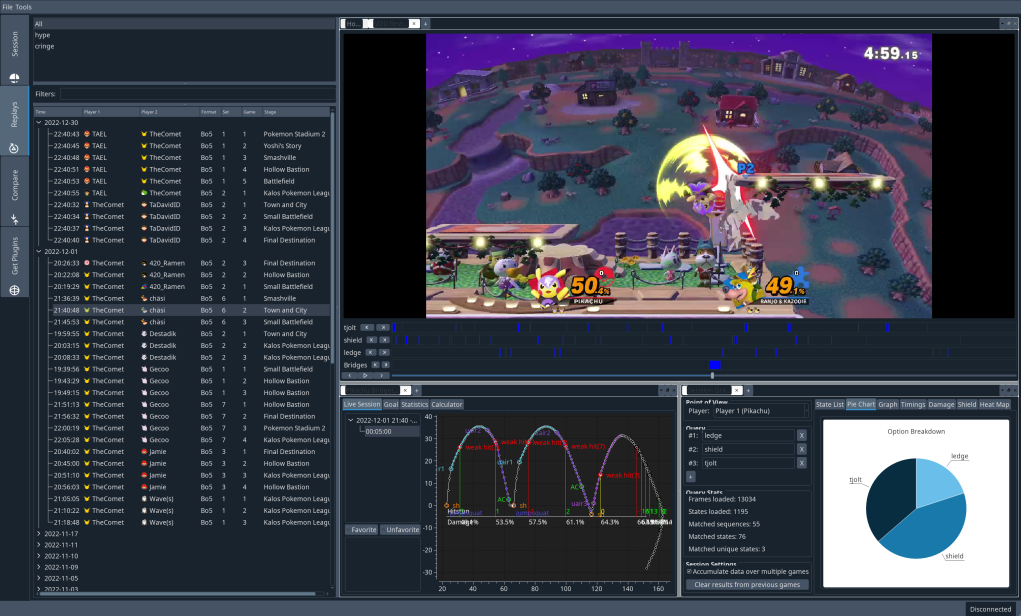
\includegraphics[width=.9\linewidth]{img/reframed.png}
	\end{figure}
	\url{https://github.com/reframedultimate/ReFramed}
	\url{https://github.com/TheComet/VODHound}
\end{frame}

\begin{frame}{You are doing trees wrong! -- Motivation}
	\begin{figure}
		\begin{tikzpicture}
			\node at (0,0)   {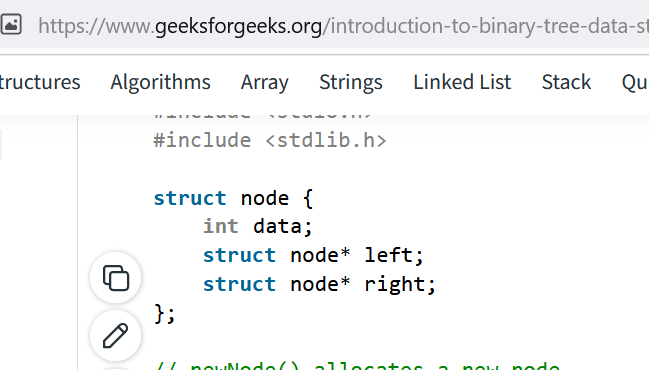
\includegraphics[width=.5\linewidth]{img/wrong2.png}};
		\end{tikzpicture}
	\end{figure}
\end{frame}

\begin{frame}{You are doing trees wrong! -- Motivation}
	\begin{figure}
		\begin{tikzpicture}
			\node at (0,0)   {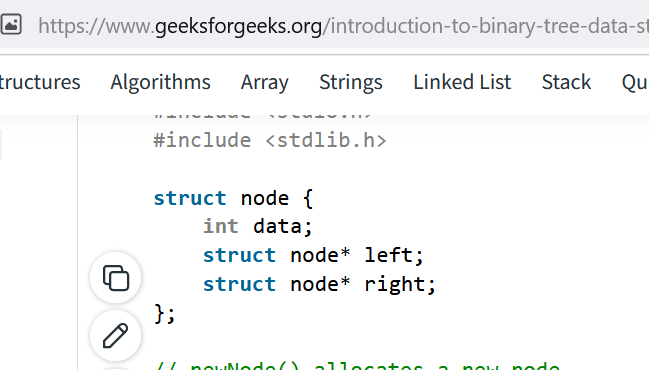
\includegraphics[width=.5\linewidth]{img/wrong2.png}};
			\node at (1,-1) {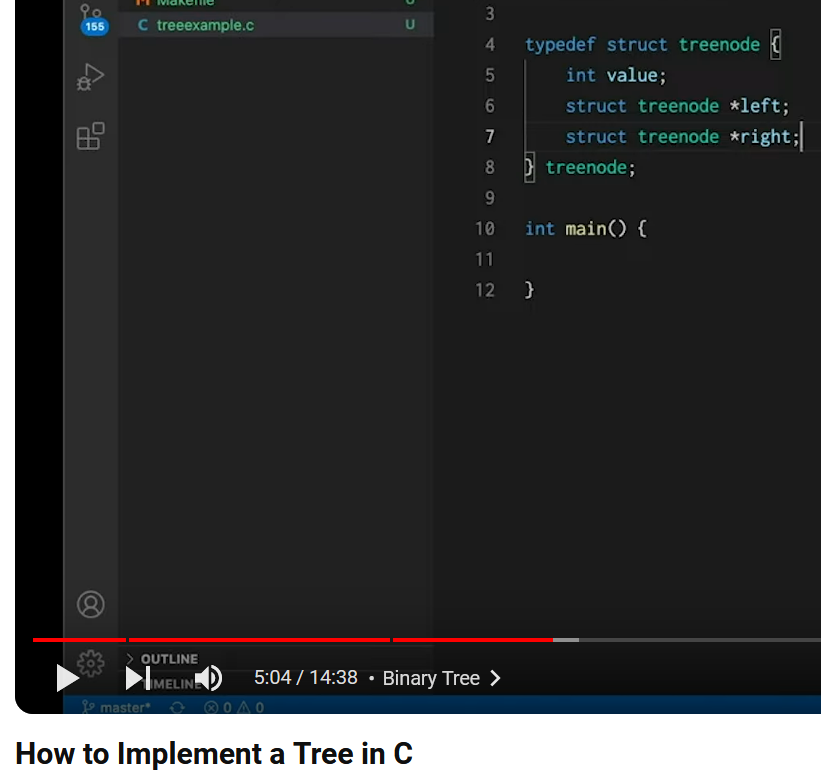
\includegraphics[width=.5\linewidth]{img/wrong1.png}};
		\end{tikzpicture}
	\end{figure}
\end{frame}

\begin{frame}{You are doing trees wrong! -- Motivation}
	\begin{figure}
		\begin{tikzpicture}
			\node at (0,0)   {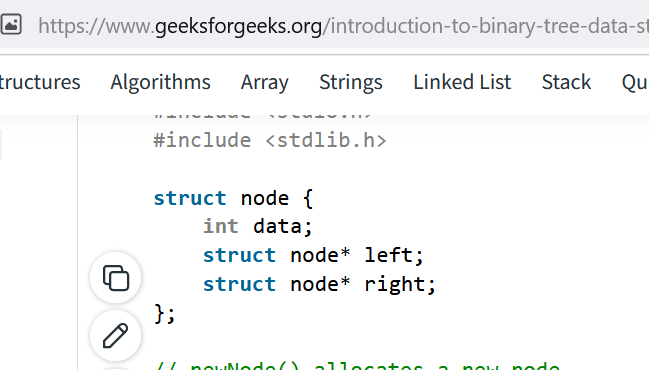
\includegraphics[width=.5\linewidth]{img/wrong2.png}};
			\node at (1,-1) {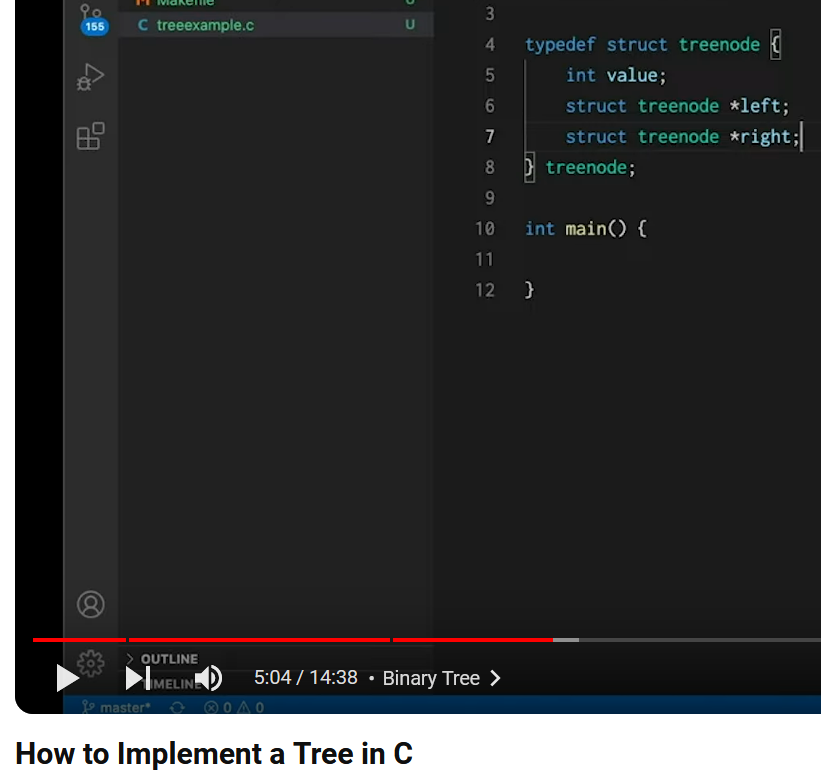
\includegraphics[width=.5\linewidth]{img/wrong1.png}};
			\node at (2,-2) {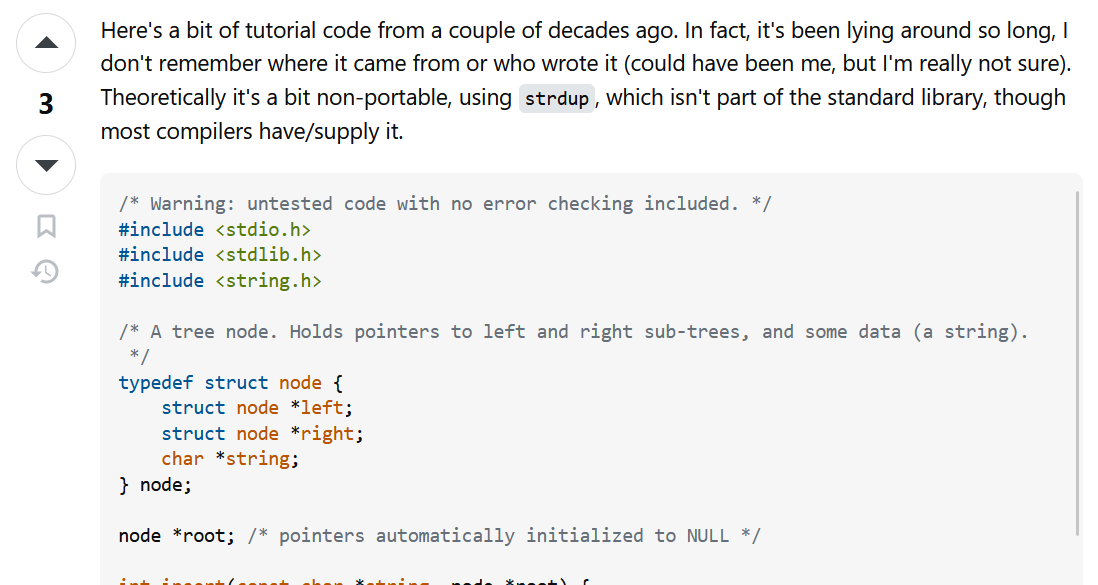
\includegraphics[width=.5\linewidth]{img/wrong4.png}};
		\end{tikzpicture}
	\end{figure}
\end{frame}

\begin{frame}{You are doing trees wrong! -- Motivation}
	\begin{figure}
		\begin{tikzpicture}
			\node at (0,0)   {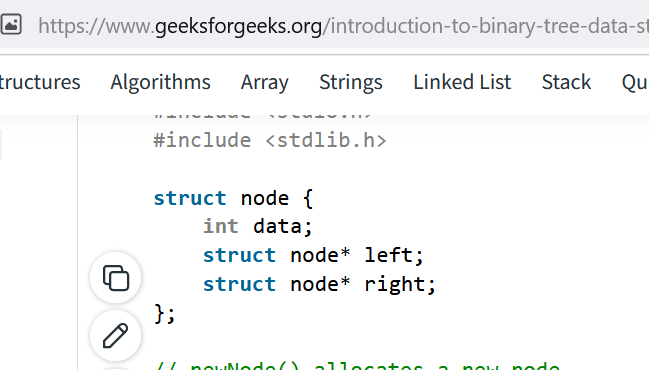
\includegraphics[width=.5\linewidth]{img/wrong2.png}};
			\node at (1,-1) {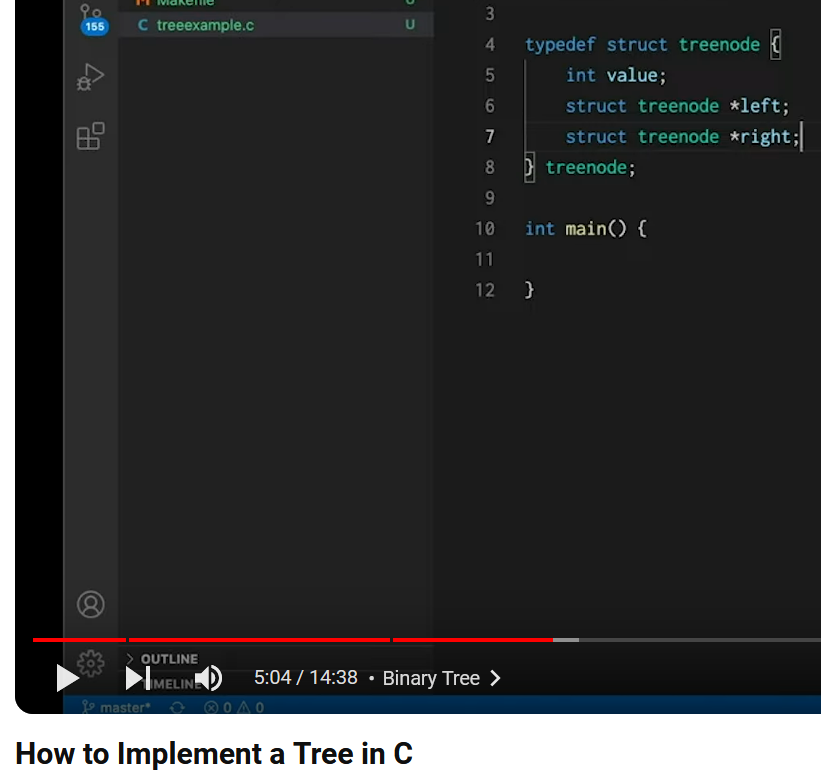
\includegraphics[width=.5\linewidth]{img/wrong1.png}};
			\node at (2,-2) {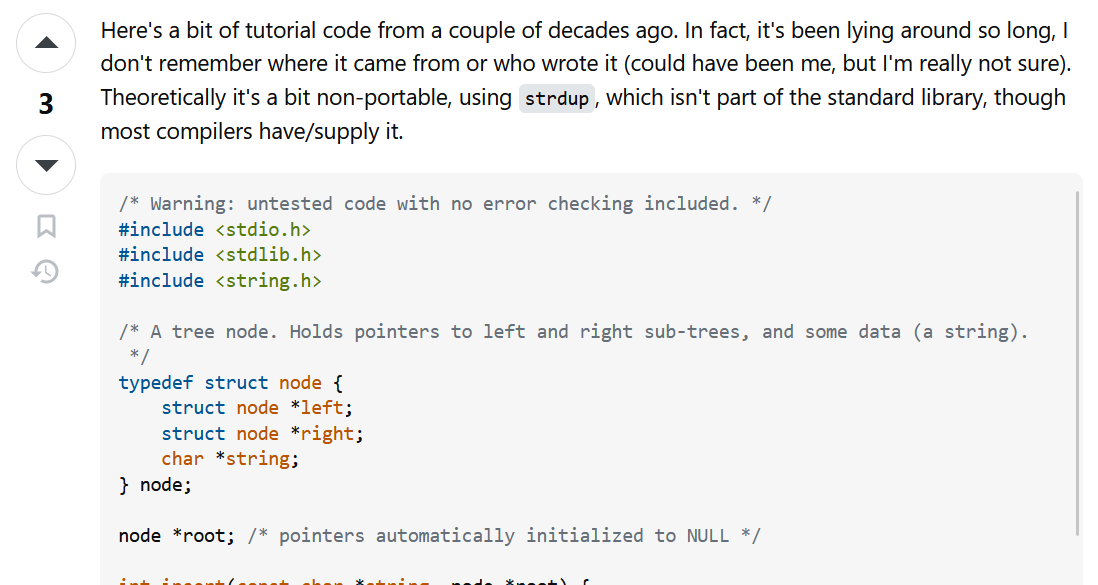
\includegraphics[width=.5\linewidth]{img/wrong4.png}};
			\node at (3,-3) {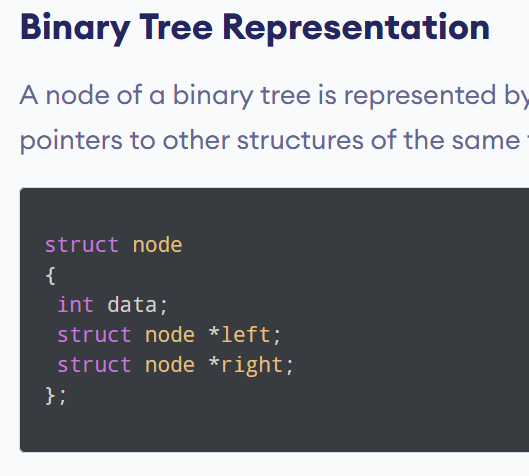
\includegraphics[width=.5\linewidth]{img/wrong3.png}};
		\end{tikzpicture}
	\end{figure}
\end{frame}

\begin{frame}{You are doing trees wrong!}
	\begin{columns}[c]
		\uncover<1-2>{
			\begin{column}[t]{.5\linewidth}{\textbf{Naive Way}}
				\lstinputlisting{c/naive.c}
			\end{column}
		}
		\uncover<2-2>{
			\begin{column}[t]{.5\linewidth}{\textbf{Better\textsuperscript{TM} Way}}
				\lstinputlisting{c/new.c}
			\end{column}
		}
	\end{columns}
\end{frame}

\begin{frame}{You are doing trees wrong! -- Memory Layout}
	\centering

	\begin{columns}[c]
		\begin{column}{.5\linewidth}{\textbf{Naive Way}}
			\lstinputlisting{c/naive.c}
		\end{column}
		\begin{column}{.5\linewidth}{}
			\begin{figure}
			\resizebox{.9\linewidth}{!}{
				\digraph{tree1}{
					graph [pad="0"];
					a->b [label="left"];
					a->c [label="right"];
				}
			}
			\end{figure}
		\end{column}
	\end{columns}

	\resizebox{\linewidth}{!}{
		\digraph{mem11}{
			rankdir=LR;
			graph [ranksep="0"];
			a [shape="rect", label="a"];
			x1 [shape="rect", label="..."];
			b [shape="rect", label="b"];
			x2 [shape="rect", label="..."];
			c [shape="rect", label="c"];
			a->x1->b->x2->c [style="invis"];
		}
	}
\end{frame}

\begin{frame}{You are doing trees wrong! -- Memory Layout}
	\centering

	\begin{columns}[c]
		\begin{column}{.5\linewidth}{\textbf{Naive Way}}
			\lstinputlisting{c/naive.c}
		\end{column}
		\begin{column}{.5\linewidth}{}
			\begin{figure}
			\resizebox{.9\linewidth}{!}{
				\digraph{tree1}{
					graph [pad="0"];
					a->b [label="left"];
					a->c [label="right"];
				}
			}
			\end{figure}
		\end{column}
	\end{columns}

	\resizebox{\linewidth}{!}{
		\digraph{mem12}{
			rankdir=LR;
			graph [ranksep="0"];
			a [shape="rect", label="a"];
			x1 [shape="rect", label="..."];
			b [shape="rect", label="b"];
			x2 [shape="rect", label="..."];
			c [shape="rect", label="c"];
			a->x1->b->x2->c [style="invis"];
			edge[style=solid, constraint=false];
			a->b;
			a->c;
		}
	}
\end{frame}

\begin{frame}{You are doing trees wrong! -- Memory Layout}
	\centering

	\begin{columns}[c]
		\begin{column}{.5\linewidth}{\textbf{Better\textsuperscript{TM} Way}}
			\lstinputlisting{c/new.c}
		\end{column}
		\begin{column}{.5\linewidth}{}
			\begin{figure}
			\resizebox{.9\linewidth}{!}{
				\digraph{tree1}{
					graph [pad="0"];
					a->b [label="left"];
					a->c [label="right"];
				}
			}
			\end{figure}
		\end{column}
	\end{columns}

	\resizebox{\linewidth}{!}{
		\digraph{mem21}{
			rankdir=LR;
			graph [ranksep="0"];
			a [shape="record", label="a|{1|2}"];
			b [shape="record", label="b|{-1|-1}"];
			c [shape="record", label="c|{-1|-1}"];
			x1 [shape="record", label="...|{|}"];
			a->b->c->x1 [style="invis"];
		}
	}
\end{frame}

\begin{frame}{You are doing trees wrong! -- Memory Layout}
	\centering

	\begin{columns}[c]
		\begin{column}{.5\linewidth}{\textbf{Better\textsuperscript{TM} Way}}
			\lstinputlisting{c/new.c}
		\end{column}
		\begin{column}{.5\linewidth}{}
			\begin{figure}
			\resizebox{.9\linewidth}{!}{
				\digraph{tree1}{
					graph [pad="0"];
					a->b [label="left"];
					a->c [label="right"];
				}
			}
			\end{figure}
		\end{column}
	\end{columns}

	\resizebox{\linewidth}{!}{
		\digraph{mem22}{
			rankdir=LR;
			graph [ranksep="0"];
			a [shape="record", label="a|{1|2}"];
			b [shape="record", label="b|{-1|-1}"];
			c [shape="record", label="c|{-1|-1}"];
			x1 [shape="record", label="...|{|}"];
			a->b->c->x1 [style="invis"];
			edge[style=solid, constraint=false];
			a->b [headport=s, tailport=sw];
			a->c [headport=s, tailport=se];
		}
	}
\end{frame}

\begin{frame}{You are doing trees wrong! -- Insert}
	\begin{columns}[c]
		\uncover<1-2>{
			\begin{column}[t]{.5\linewidth}{\textbf{Naive Way}}
				\lstinputlisting[basicstyle=\ttfamily\scriptsize]{c/insert-naive.c}
			\end{column}
		}
		\uncover<2-2>{
			\begin{column}[t]{.5\linewidth}{\textbf{Better\textsuperscript{TM} Way}}
				\lstinputlisting[basicstyle=\ttfamily\scriptsize]{c/insert-new.c}
			\end{column}
		}
	\end{columns}
\end{frame}

\begin{frame}{You are doing trees wrong! -- Insert}
	\begin{columns}[c]
		\begin{column}[t]{.5\linewidth}{\textbf{Naive Way}}
			\lstinputlisting[basicstyle=\ttfamily\scriptsize]{c/insert-naive.c}
		\end{column}
		\begin{column}[t]{.5\linewidth}{\textbf{Better\textsuperscript{TM} Way}}
			\lstinputlisting[basicstyle=\ttfamily\scriptsize]{c/insert-new2.c}
		\end{column}
	\end{columns}
\end{frame}

\begin{frame}{You are doing trees wrong! -- Insert}
	\begin{columns}[c]
		\begin{column}[t]{.5\linewidth}{\textbf{Naive Way}}
			\lstinputlisting[basicstyle=\ttfamily\scriptsize]{c/insert-naive2.c}
		\end{column}
		\begin{column}[t]{.5\linewidth}{\textbf{Better\textsuperscript{TM} Way}}
			\lstinputlisting[basicstyle=\ttfamily\scriptsize]{c/insert-new3.c}
		\end{column}
	\end{columns}
\end{frame}

\begin{frame}{You are doing trees wrong! -- Insert Performance}
	\begin{figure}
		\centering
		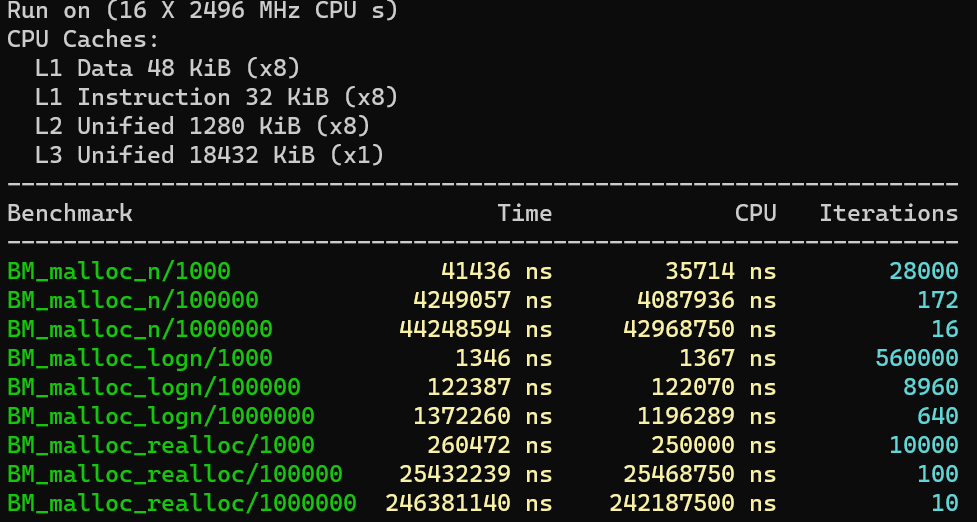
\includegraphics[width=\linewidth]{img/benchmarks.png}
	\end{figure}
\end{frame}

\begin{frame}{You are doing trees wrong! -- Find}
	\begin{columns}[c]
		\uncover<1-2>{
			\begin{column}[t]{.5\linewidth}{\textbf{Naive Way}}
				\lstinputlisting[basicstyle=\ttfamily\scriptsize]{c/find-naive.c}
			\end{column}
		}
		\uncover<2-2>{
			\begin{column}[t]{.5\linewidth}{\textbf{Better\textsuperscript{TM} Way}}
				\lstinputlisting[basicstyle=\ttfamily\scriptsize]{c/find-new-dfs.c}
			\end{column}
		}
	\end{columns}
\end{frame}

\begin{frame}{You are doing trees wrong! -- Find}
	\begin{columns}[c]
		\begin{column}[t]{.5\linewidth}{\textbf{Naive Way}}
			\lstinputlisting[basicstyle=\ttfamily\scriptsize]{c/find-naive.c}
		\end{column}
		\begin{column}[t]{.5\linewidth}{\textbf{Better\textsuperscript{TM} Way}}
			\lstinputlisting[basicstyle=\ttfamily\scriptsize]{c/find-new.c}
		\end{column}
	\end{columns}
\end{frame}

\begin{frame}{You are doing trees wrong! -- Delete Node}
	\begin{columns}[c]
		\uncover<1-2>{
			\begin{column}[t]{.5\linewidth}{\textbf{Naive Way}}
				\lstinputlisting[basicstyle=\ttfamily\scriptsize]{c/del-naive.c}
			\end{column}
		}
		\uncover<2-2>{
			\begin{column}[t]{.5\linewidth}{\textbf{Better\textsuperscript{TM} Way}}
				\lstinputlisting[basicstyle=\ttfamily\scriptsize]{c/del-new.c}
			\end{column}
		}
	\end{columns}
\end{frame}

\begin{frame}{You are doing trees wrong! -- Delete Tree}
	\begin{columns}[c]
		\uncover<1-2>{
			\begin{column}[t]{.5\linewidth}{\textbf{Naive Way}}
				\lstinputlisting[basicstyle=\ttfamily\scriptsize]{c/del-naive.c}
			\end{column}
		}
		\uncover<2-2>{
			\begin{column}[t]{.5\linewidth}{\textbf{Better\textsuperscript{TM} Way}}
				\lstinputlisting[basicstyle=\ttfamily\scriptsize]{c/del-new-tree.c}
			\end{column}
		}
	\end{columns}
\end{frame}

\begin{frame}{You are doing trees wrong! -- (De-)Serialization}
	\begin{columns}[c]
		\uncover<1-2>{
			\begin{column}[t]{.5\linewidth}{\textbf{Naive Way}}
				\lstinputlisting[basicstyle=\ttfamily\tiny]{c/ser-naive.c}
			\end{column}
		}
		\uncover<2-2>{
			\begin{column}[t]{.5\linewidth}{\textbf{Better\textsuperscript{TM} Way}}
				\lstinputlisting[basicstyle=\ttfamily\scriptsize]{c/ser-new.c}
			\end{column}
		}
	\end{columns}
\end{frame}

\begin{frame}{You are doing trees wrong! -- Summary}
	\begin{columns}[c]
		\begin{column}[t]{.5\linewidth}{\textbf{Pros}}
			\begin{itemize}
				\uncover<2-6>{\item More opportunities for tuning performance}
				\uncover<3-6>{\item Faster (fewer memory allocations)}
				\uncover<4-6>{\item Less memory consumption}
				\uncover<5-6>{\item Higher cache locality}
				\uncover<6-6>{\item Recursion is not always necessary! Opportunity for more efficient algorithms}
			\end{itemize}
		\end{column}
		\begin{column}[t]{.5\linewidth}{\textbf{Cons}}
			\begin{itemize}
				\uncover<1-6>{\item More memory management overhead}
			\end{itemize}
		\end{column}
	\end{columns}
\end{frame}

\begin{frame}[c]{}
	\centering
	\Large{Thank you!}
	\normalsize{\url{https://github.com/TheComet/do-trees-right}}
\end{frame}

\end{document}
